\documentclass{article}
\usepackage[UTF8,space,hyperref]{ctex}
\usepackage{amsmath, amsthm, amssymb, bm, color, framed, graphicx, mathrsfs, physics}
\usepackage[breaklinks, colorlinks]{hyperref}
\usepackage{wrapfig}
\usepackage{caption}
\usepackage{geometry}
\hypersetup{hidelinks} 
\title{矩阵乘法优化报告\\ \large 汇编语言第二次大作业}
\author{石曜铭}
\date{\today}

\geometry{left = 4cm, right = 4cm, top = 3cm, bottom = 3cm}

\begin{document}

\maketitle


\section{实验整体设计}

本实验探究矩阵乘法从朴素实现到底层优化的不同写法,并根据运行时间等结果分析各种优化的作用。

本实验一共探究了六种写法:
\begin{enumerate}
\item python 朴素实现;
\item C 语言朴素实现;
\item 在 2 的基础上,添加多线程优化;
\item 在 3 的基础上,考虑 cache 局部性机制,使用分块优化;
\item 在 4 的基础上,使用SIMD向量指令优化;
\item 在 5 的基础上,使用其他优化方法。这里使用比 5 向量化程度更高的 AVX512 实现。
\end{enumerate}

因此实验包含矩阵乘法的多种实现方式,为了验证它们的正确性,我使用 python 的 numpy 包进行答案的计算,并以之为标准与其他方法的输出进行比较,精度不低于 $10^{-5}$ 。

为了优化效果的普遍性,实验在 $5$ 个不同计算机上进行了测试。具体结果见“效果分析”一节。

\textbf{注:}本实验中随机矩阵的方式是使用 C 语言中的 $\texttt{rand}$ 函数,并将结果除以 $\texttt{RAND\_MAX}$ 得到一个 $0\sim 1$ 之间的浮点数,使用 $\texttt{double}$ 存储。

\section{源码分析}

\subsection{代码结构}

\begin{wrapfigure}{r}[0cm]{0pt}
  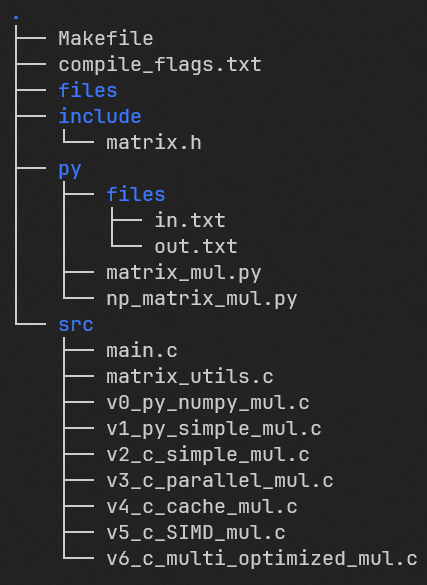
\includegraphics[width=0.4\textwidth]{pics/structure.png}
  \caption*{代码结构图}
\end{wrapfigure}

如右图,整体由一个头文件和多个C语言代码文件和 py 脚本构成。$\texttt{matrix.h}$ 定义了结构体 $\texttt{Matrix}$,为了内存连续,降低后续 SIMD 优化中被编译器认为不可优化的可能性,在这里使用一维数组存储矩阵,并在堆区开辟内存。

$\texttt{matrix\_utils.c}$ 主要包含一些矩阵的基本操作,比如输入输出。其他七个文件从 $\texttt{v0}$ 到 $\texttt{v6}$ 分别是不同写法的矩阵乘法实现。接下来逐一进行源码分析。

\subsection{python 朴素实现以及调用 NumPy 库得到标准}

python 的朴素实现在 $\texttt{v1}$ 中。本实验通过系统调用来调用 py 脚本。首先将矩阵输出到指定文件,然后进行 py 脚本的调用。

\begin{figure}[htbp]
  \centering
  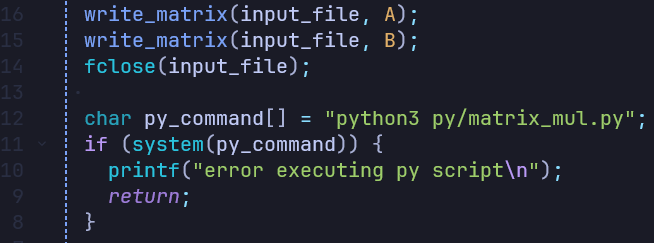
\includegraphics[width=0.8\textwidth]{pics/v1code.png}
  \caption*{输出矩阵并调用py脚本}
\end{figure}

朴素实现的 python 矩阵乘法核心代码:
\begin{figure}[htbp]
  \centering
  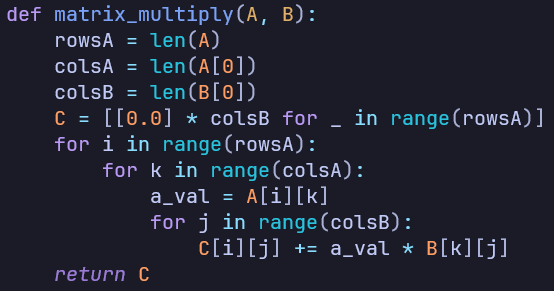
\includegraphics[width=0.65\textwidth]{pics/python_simple.png}
  \caption*{python 矩阵乘法}
\end{figure}

调用 NumPy 库代码:$\texttt{C = np.dot(A, B)}.$

\subsection{C 语言朴素实现}

朴素实现的三重循环是可以调换顺序的。这里为了减少 cache miss,选择先枚举 $A$ 的行,再枚举 $A$ 的列,然后枚举 $B$ 的列。这样是在内部循环中是连续访问 $B$ 中元素的,减少了 cache miss。
\begin{figure}[htbp]
  \centering
  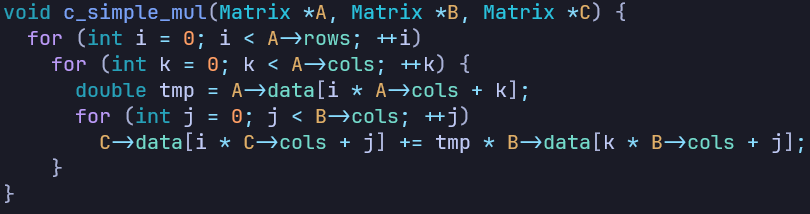
\includegraphics[width=0.8\textwidth]{pics/v2code.png}
  \caption*{C 语言朴素矩阵乘法}
\end{figure}

\subsection{多线程优化}

首先确定要将对 $A$ 不同行之间的处理并行,默认线程数是 $8$。根据线程数对行进行分块,然后使用统一的线程工作函数计算对应的矩阵乘法结果,然后进行合并。
\begin{figure}[htbp]
  \centering
  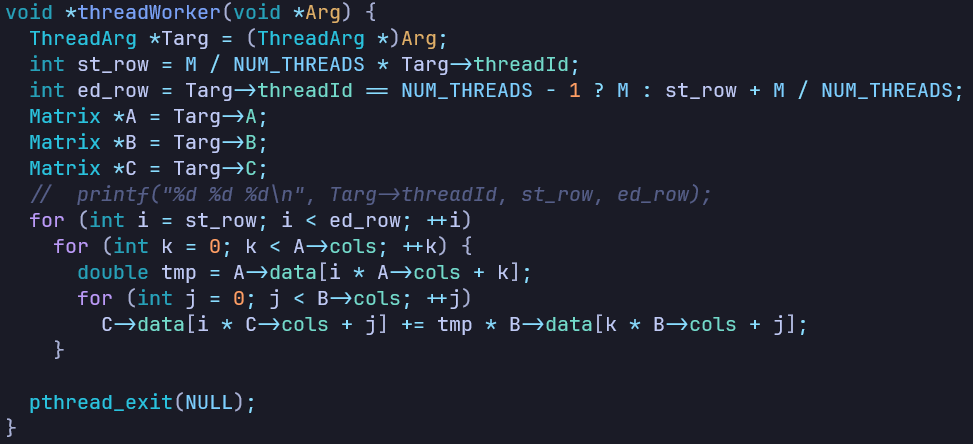
\includegraphics[width=0.7\textwidth]{pics/v3code_1.png}
  \caption*{线程工作函数}
\end{figure}

\begin{figure}[htbp]
  \centering
  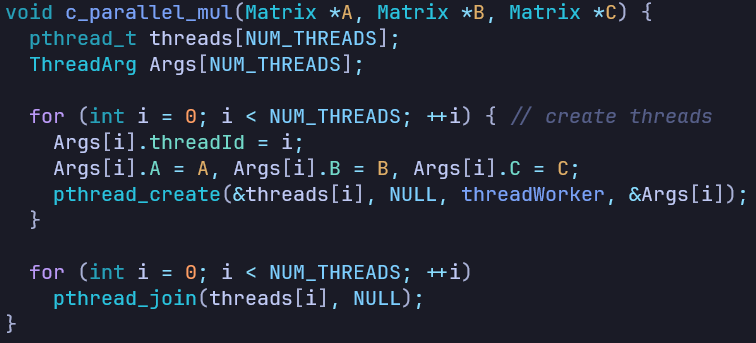
\includegraphics[width=0.7\textwidth]{pics/v3code_2.png}
  \caption*{线程的创建}
\end{figure}

\subsection{利用 cache 进行分块优化}
在矩阵乘法的过程中,将矩阵拆成能放进 L1-Cache 的小块,可以进一步降低 cache miss,增加加载速度。所以需要根据 L1-Cache 的大小计算出合适的 block 大小。

在分块矩阵乘法的多线程实现中,为了尽可能多的利用闲置的线程,使用动态分配的方法。即对每个线程记录一个指向原子操作的整型代表下一个要处理的行。哪个线程先处理完,就可以给这个原子操作的整型加上 $\texttt{block\_size}$ 。

\begin{figure}[htbp]
  \centering
  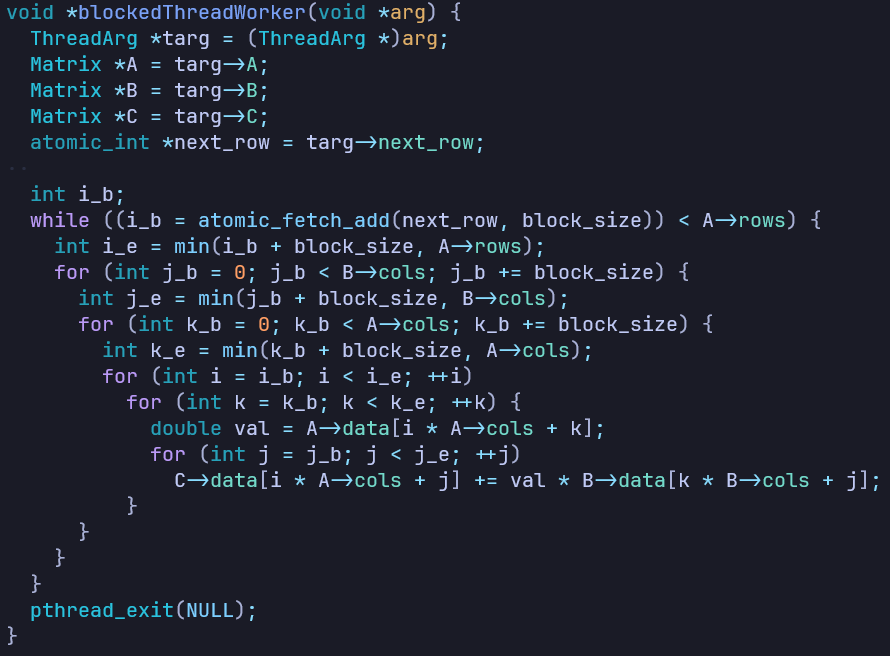
\includegraphics[width=0.8\textwidth]{pics/v4code.png}
  \caption*{分块矩阵乘法的线程函数}
\end{figure}


\subsection{使用 SIMD 指令优化}

为了能使编译器做出向量化的优化,需要在代码中给出明确的标志表示这里可以被向量化,比如循环展开。将循环变量每次加 $4$,一次循环中处理 $4$ 个乘加操作。但是,经过多次尝试,编译器始终认为这里的指针可能存在地址上的重叠和别名,只会做出 SSE 优化,即使用 $128$ 位的 $\texttt{xmm}$ 寄存器,每次处理两个乘加操作。即使使用 $\texttt{restrict}$ 关键字修饰也不能做到。

解决方案是,强行在代码中使用 $\texttt{immintrin.h}$  中的内联函数,直接显式声明一个使用 $\texttt{ymm}$ 寄存器的变量,然后进行操作。

此版本和 $4$ 的区别仅在于最内层循环的函数有所改变:
\begin{figure}[htbp]
  \centering
  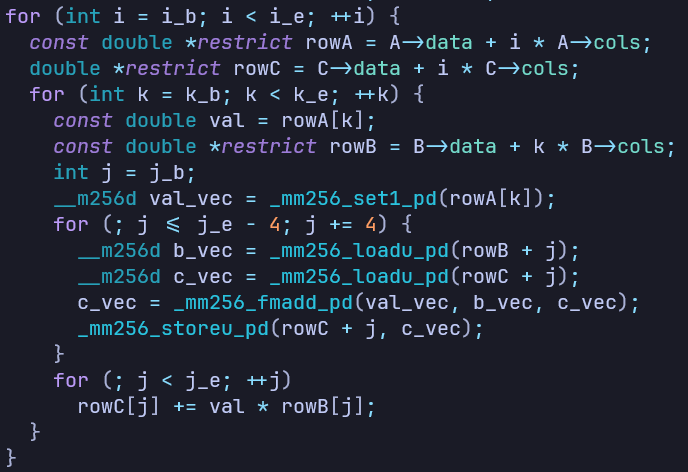
\includegraphics[width=0.6\textwidth]{pics/v5code.png}
  \caption*{显式使用 AVX}
\end{figure}

\begin{figure}[htbp]
  \centering
  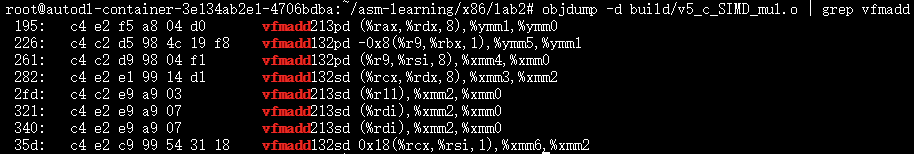
\includegraphics[width=0.7\textwidth]{pics/simd_check.png}
  \caption*{通过 objdump 确认使用了 AVX}
\end{figure}

\vspace{0.7cm}
\subsection{使用 AVX512 优化}

有些 CPU 可以使用 AVX512 实现更高程度的向量化,因此可以将 $5$ 中的 $256$ 位的内联函数改为对应的 $512$ 位。需加入 $\texttt{-mavx512f -mavx512dq}$ 编译选项。

此版本和 $5$ 的区别仅在于最内层循环的函数有所改变:


\begin{figure}[htbp]
  \centering
  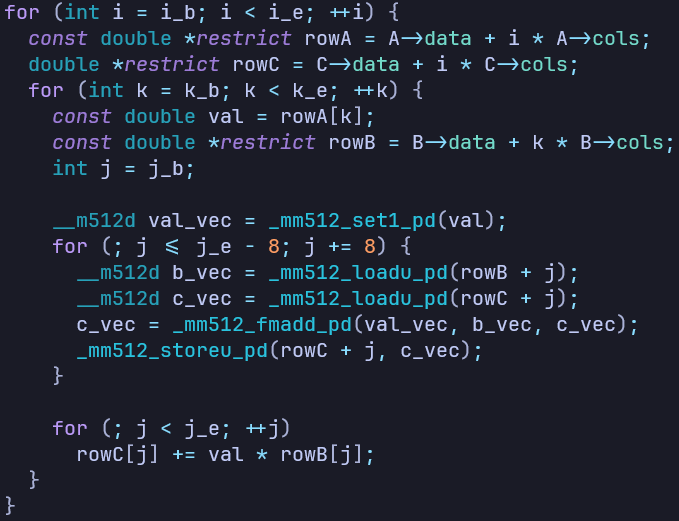
\includegraphics[width=0.57\textwidth]{pics/v6code.png}
  \caption*{显式使用 AVX512}
\end{figure}

\begin{figure}[htbp]
  \centering
  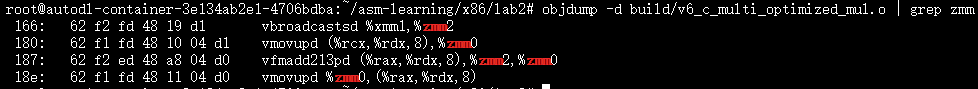
\includegraphics[width=0.8\textwidth]{pics/avx512_check.png}
  \caption*{通过 objdump 确认使用了 AVX512}
\end{figure}

\section{效果分析}
\label{section:3}

实验一共在 $5$ 台基于不同硬件的计算机中进行测试。以下为五台计算机CPU的型号:

\begin{center}
\begin{tabular}{c|c}
\textbf{序号} & \textbf{CPU型号} \\
\hline 
1 & AMD Ryzen 9 8940HX \\ 
2 & 13th Gen Intel(R) Core(TM) i9-13900H \\ 
3 & 11th Gen Intel(R) Core(TM) i5-1135G7 2.40GHz \\ 
4 & 12th Gen Intel(R) Core(TM) i9-12900H 2.50Ghz \\
5 & Intel(R) Xeon(R) Platinum 8470Q  \\ 
\end{tabular}
\end{center}

以下为运行结果:
\begin{center}
\begin{tabular}{c|c|c|c|c|c|c|c}
\textbf{序号} & \textbf{NumPy} & \textbf{v1} & \textbf{v2} & \textbf{v3} & \textbf{v4} & \textbf{v5} & \textbf{v6} \\
\hline 
1 & 12358 & 2767098 & 40564 & 5512 & 3959 & 1533 & 1763 \\ 
2 & 135141 & $\sim$ 3600000  & 90091 & 16824 & 20477 & 12396 & 不支持 \\ 
3 & 20115 & $\sim$ 3600000 & 42991 & 16812 & 12785 & 7166 & 6501 \\ 
4 & 12476 & 1895516 & 37861 & 7441 & 4235 & 2186 & 不支持 \\
5 & 18135 & 3232503 & 66255 & 11103 & 5335 & 2436 & 2584 \\ 
\end{tabular}
\end{center}

相对 v2 的加速比:
\begin{center}
\begin{tabular}{c|c|c|c|c}
\textbf{序号} & \textbf{v3} & \textbf{v4} & \textbf{v5} & \textbf{v6} \\
\hline 
1 & 7.36 & 10.25 & 26.45 & 23.01 \\ 
2 & 5.35 & 4.40 & 7.27 & 不支持 \\ 
3 & 2.56 & 3.36 & 6.00 & 6.61 \\ 
4 & 5.09 & 8.94 & 17.31 & 不支持 \\
5 & 5.97 & 12.42 & 27.20 & 25.64 \\ 
\end{tabular}
\end{center}

由结果可见,这些写法的速度基本上呈现递增的趋势。当然,也能注意到一些反常现象比如在 $2$ 号上分块多线程比不分块要慢,这可能是 $\texttt{block\_size}$ 大小过大导致的。另外,还能够发现,对于一些比较新的 CPU,AVX512比256反而更慢一些,这可能是因为 AVX512 指令集的设计没有跟上硬件的迭代更新。


\section{备注}

本实验代码仓库已经上传到\href{https://github.com/Symmetryagain/asm-learning/tree/main}{github}上,在x86/lab2目录下。
\end{document}